\documentclass[10pt, a4paper]{article}
\usepackage[T1]{fontenc}
\usepackage[left=2cm, right=2cm, top=2cm, bottom=2cm]{geometry}
\usepackage{graphicx}
\usepackage{mathtools}
\usepackage{amssymb}
%\usepackage{mathrsfs} % to use \mathscr{...}
\usepackage{xcolor} % \textcolor{red}{...} & \mathcolor{red}{...}
\usepackage{nameref}
\usepackage{hyperref} %Automatically links \label and \ref commands; Always load last
\hypersetup{
	linktocpage,
	colorlinks=true, % false: boxed links; true: colored links
	linkcolor=red, % color of internal links
	citecolor=blue, % color of links to bibliography
	filecolor=magenta, % color of file links
	urlcolor=purple % color of external links
} % hidelinks
%----------------------------------------------------------------------
\usepackage{xeCJK}
\setCJKmainfont{GenRyuMin2 JP} % 源流明体
\setCJKmonofont{GenRyuMin2 JP} % font used in \texttt{} (just to prevent a warning)
%----------------------------------------------------------------------
% to handle a large project
%\usepackage{import}
%----------------------------------------------------------------------
\usepackage{indentfirst}
\setlength{\parindent}{0em} % 首行缩进
%----------------------------------------------------------------------
% horizontal line
%\noindent\rule[0.5ex]{\linewidth}{0.5pt} % horizontal line

\usepackage{dashrule}
%\noindent\hdashrule[0.5ex]{\linewidth}{0.5pt}{1mm} % horizontal dashed line
%----------------------------------------------------------------------
\usepackage[breakable]{tcolorbox} % box with color; highlight text \colorbox{yellow}{...}
\tcbset{breakable, colback=white, colframe=green!30!black, coltext=black!60!white, fonttitle=\bfseries}

\usepackage{tabularx} % LaTeX table
\usepackage{booktabs}

\usepackage{float} % appropriate way to handle figures
% example:
%\begin{figure}[H]
%	\centering
%	\includegraphics[scale=1]{figures/file-name}
%	\caption{...}
%\end{figure}
\usepackage{subfigure}
% following David Tong's convention, one should always add a caption to figures, but not to tables.
%----------------------------------------------------------------------
\numberwithin{equation}{section}
\allowdisplaybreaks % allow page breaks inside math environments globally

\usepackage{braket}
\usepackage{cancel}

%\usepackage{leftindex}
\usepackage{tensor} % how to handle indeces: https://tex.stackexchange.com/questions/11542/left-and-right-subscript-superscript

% use \, in math environment
% except for texts embeded in math environment, use \ instead
%----------------------------------------------------------------------
% fancy title font
%\newfontfamily\fancyfont{Centaur}
%----------------------------------------------------------------------
\title{\Huge \textbf{Maps Between Manifolds}}
\author{万思扬}
\date{October 4, 2024}
%----------------------------------------------------------------------
\begin{document}
	\maketitle
	
	Email: \href{mailto:wansiyang03@gmail.com}{\texttt{wansiyang03@gmail.com}}
	
	\url{https://github.com/siyang03/my-note---maps-between-manifolds}
	
	\tableofcontents
	
	\section{a map between two manifolds}
	\begin{itemize}
		\item $\phi : M_1 \rightarrow M_2$ 是一个流形间的映射, 如下图所示,
		
		\begin{figure}[H]
			\centering
			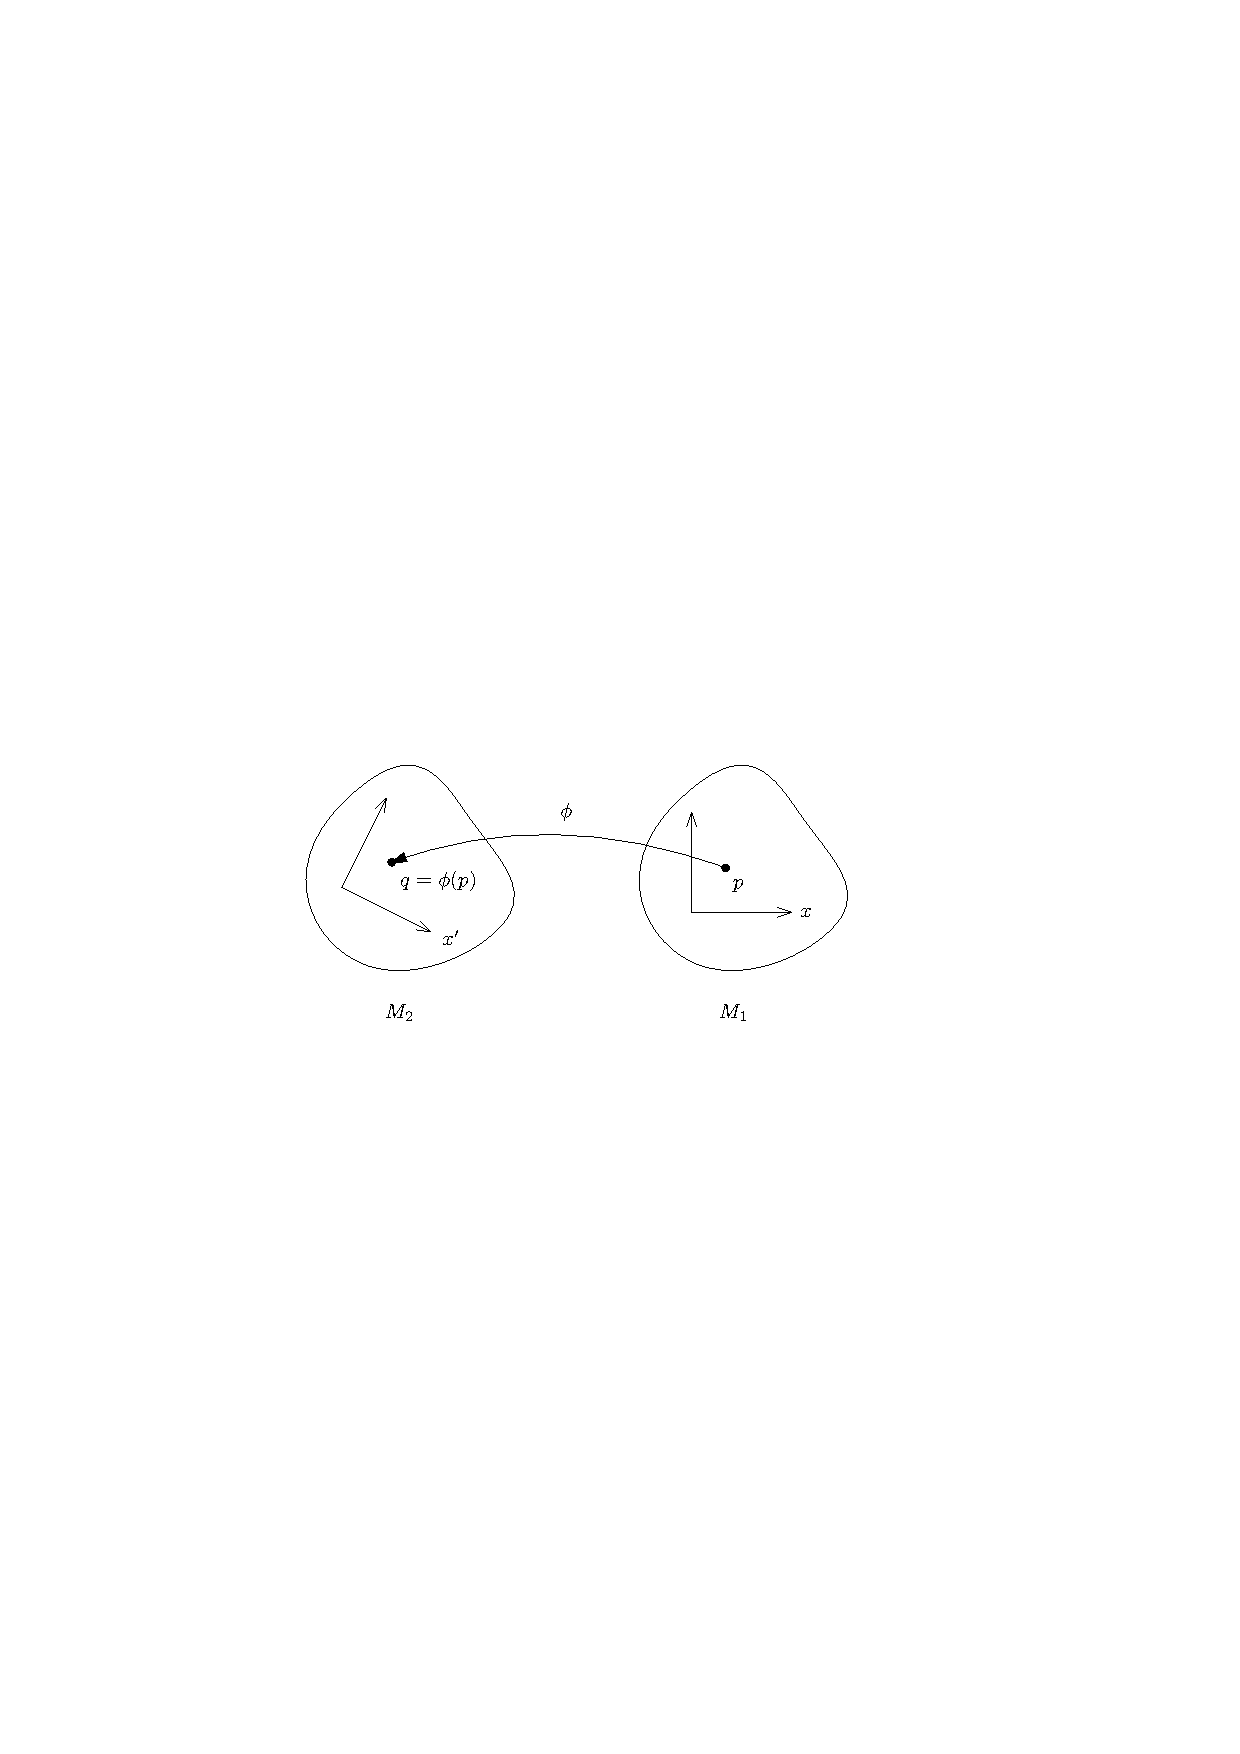
\includegraphics[scale=1]{figures/a map between two manifolds.pdf}
			\caption{a map between two manifolds}
		\end{figure}
	\end{itemize}
	
	\subsection{pull-back}
	\begin{itemize}
		\item 将 $M_2$ 上的标量场拉回得到 $M_1$ 上的标量场, 特别地,
		\begin{equation}
			x = \phi^* x' \quad \text{i.e.} \quad x'(q) = x'(\phi(p)) \mathcolor{red}{=} (\phi^* x')(p) = x(p)
		\end{equation}
		不过要注意, $\phi^* x'$ 不是 $M_1$ 上的坐标, 因为 $\phi$ 不是 one-to-one, (一个有帮助的例子是 $\dim M_2 < \dim M_1$).
	\end{itemize}
	
	\subsection{push-forward}
	\begin{itemize}
		\item 将 $M_1$ 上的矢量场推前得到 $M_2$ 上的矢量场, 特别地,
		\begin{equation}
			\phi_* \frac{\partial}{\partial x} = \frac{\partial}{\partial x'} \quad \text{i.e.} \quad \frac{\partial}{\partial x'^\mu} (x') = \Big( \phi_* \frac{\partial}{\partial x^\mu} \Big) (x') \mathcolor{red}{=} \frac{\partial}{\partial x^\mu} (\phi^* x') = \frac{\partial}{\partial x^\mu} (x)
		\end{equation}
	\end{itemize}
	
	\subsection{pull-back again}
	\begin{itemize}
		\item 将 $M_2$ 上的对偶矢量场拉回得到 $M_1$ 上的对偶矢量场, 特别地,
		\begin{equation}
			dx = \phi^* dx' \quad \text{i.e.} \quad dx'^\mu \Big( \frac{\partial}{\partial x'} \Big) = dx'^\mu \Big( \phi_* \frac{\partial}{\partial x} \Big) \mathcolor{red}{=} (\phi^* dx'^\mu) \Big( \frac{\partial}{\partial x} \Big) = dx^\mu \Big( \frac{\partial}{\partial x} \Big)
		\end{equation}
	\end{itemize}
	
	\section{some examples}
	\subsection{a simple example}
	\begin{itemize}
		\item 考虑 $\phi : \mathbb{R}^3 \rightarrow \mathbb{R}^2$, 两个流形上分别有直角坐标和极坐标, 映射具体形式为,
		\begin{equation}
			\phi(p) = q \quad \text{s.t.} \quad r(q) = x(p), \theta(q) = y(p)
		\end{equation}
		如下图所示,
		
		\begin{figure}[H]
			\centering
			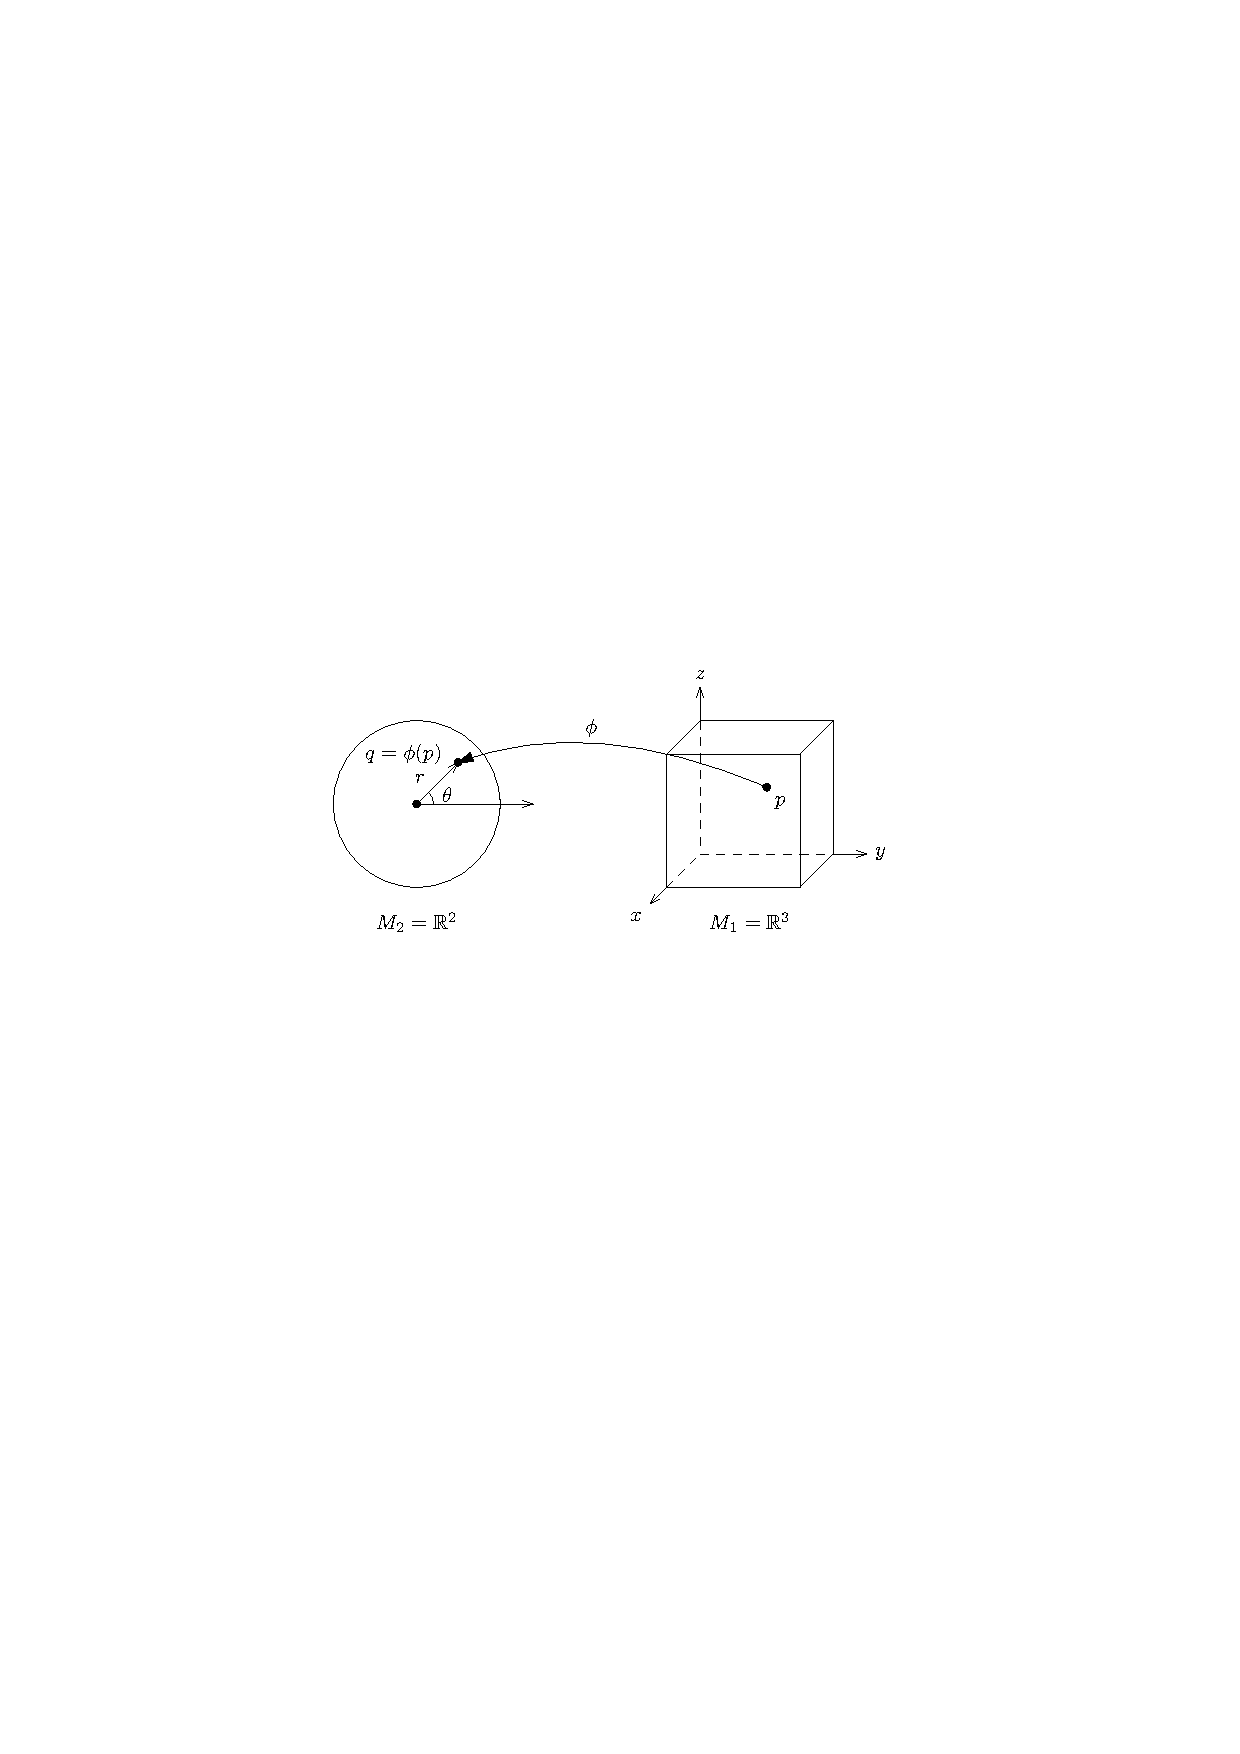
\includegraphics[scale=1]{figures/a simple example.pdf}
			\caption{a simple example}
		\end{figure}
		
		\item 此时 $x = \{x, y, z\}, x' = \{r, \theta\}$, 并且有,
		\begin{equation}
			\begin{dcases}
				x = \phi^* r \quad y = \phi^* \theta \\
				\phi_* \Big( \frac{\partial}{\partial x} + \alpha \frac{\partial}{\partial z} \Big) = \frac{\partial}{\partial r} \quad \phi_* \Big( \frac{\partial}{\partial y} + \beta \frac{\partial}{\partial z} \Big) = \frac{\partial}{\partial \theta} & \text{其中} \ \alpha, \beta \ \text{是任意实数} \\
				dx = \phi^* dr \quad dy = \phi^* d\theta
			\end{dcases}
		\end{equation}
	\end{itemize}
	
	\subsection{Lorentz transformation}
	\begin{itemize}
		\item Lorentz 变换 $\phi : M \rightarrow M$ (其中 $M = \mathbb{R}^{3, 1}$) 的具体形式为,
		\begin{equation}
			\phi : p \mapsto q \quad \text{s.t.} \quad x(q) = \Lambda^{- 1} x(p)
		\end{equation}
		如下图所示,
		
		\begin{figure}[H]
			\centering
			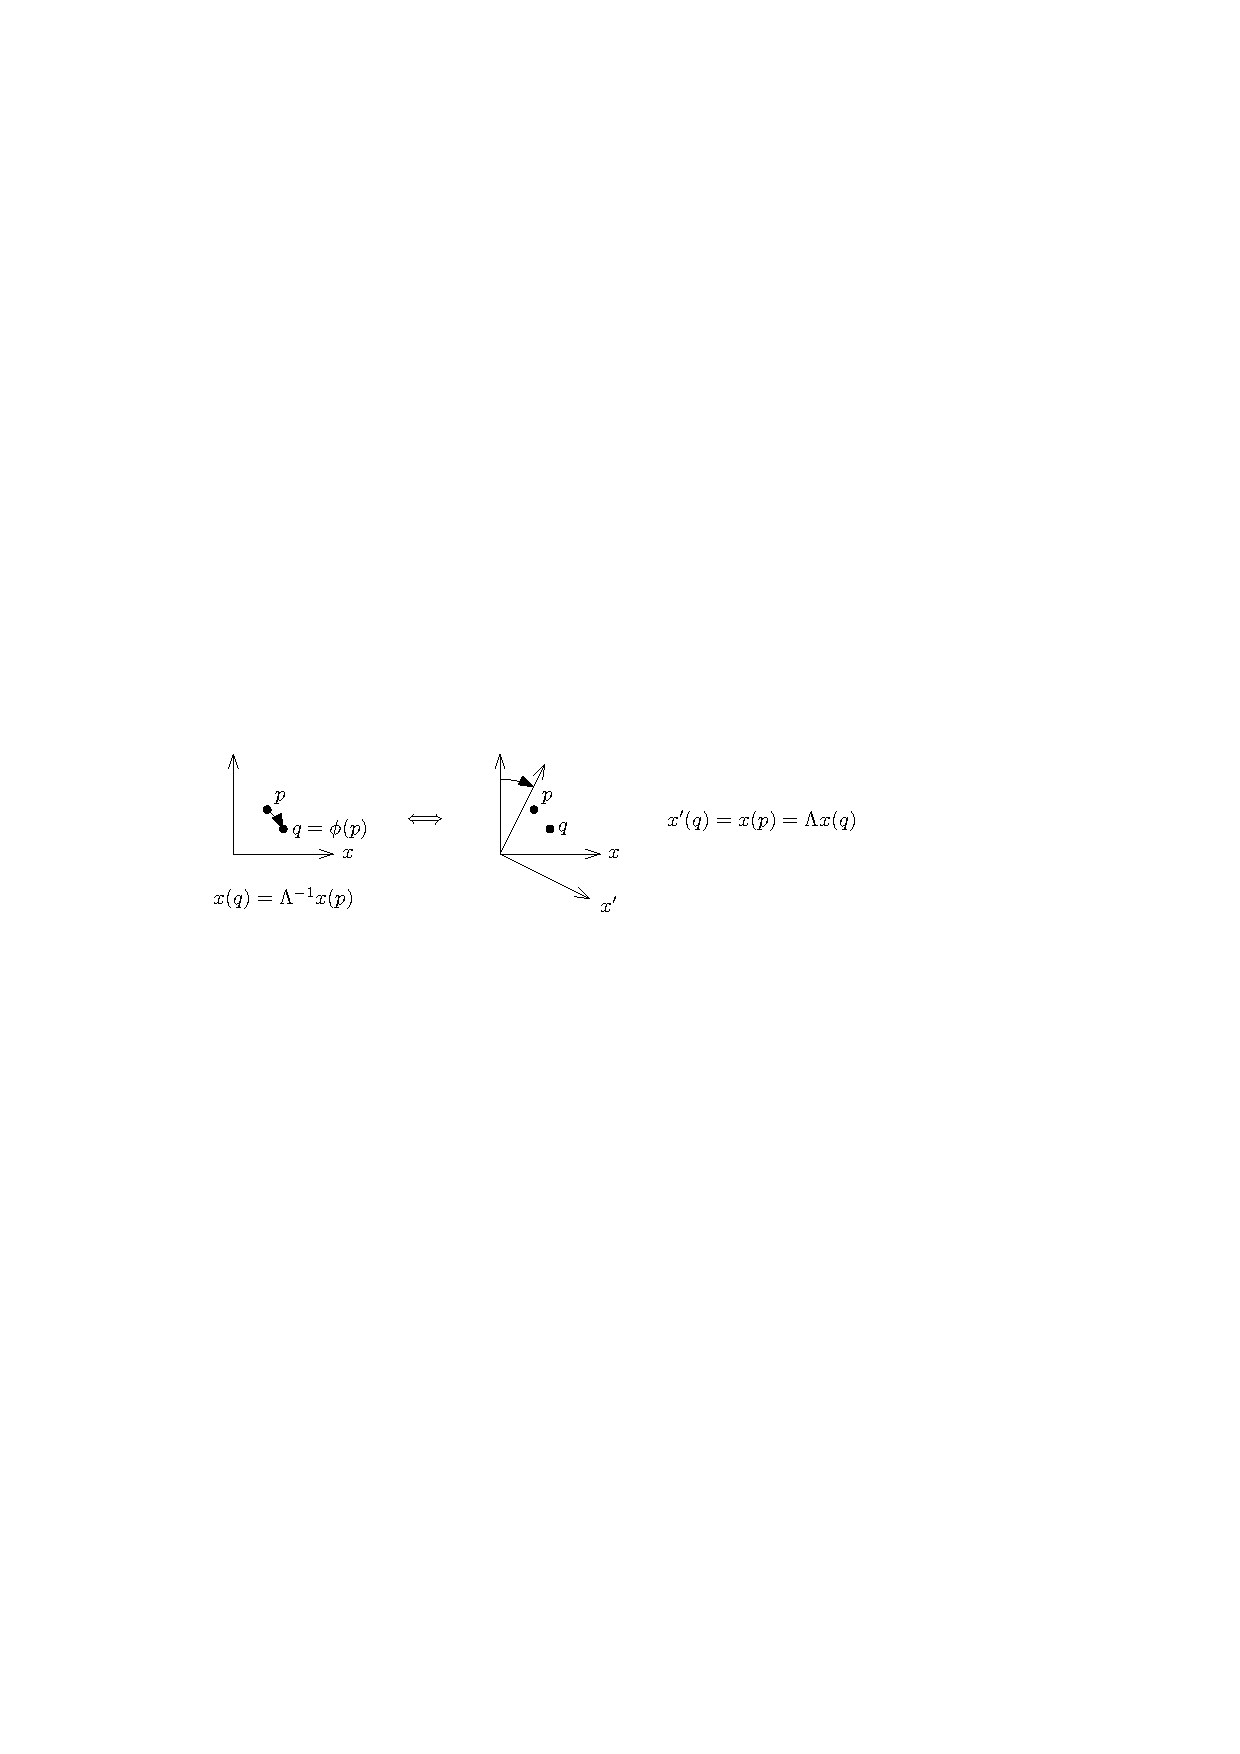
\includegraphics[scale=1]{figures/Lorentz transformation.pdf}
			\caption{Lorentz transformation}
		\end{figure}
		
		\item 有如下关系,
		\begin{equation}
			\begin{dcases}
				x = \phi^* x' = \Lambda^{- 1} x' \\
				\phi_* \frac{\partial}{\partial x} = \frac{\partial}{\partial x'} = \eta \Lambda \eta \frac{\partial}{\partial x} \\
				dx = \phi^* dx' = \Lambda^{- 1} dx'
			\end{dcases}
		\end{equation}
		
		\begin{tcolorbox}[title=calculation:]
			对于推前映射,
			\begin{equation}
				\frac{\partial}{\partial x'^\mu} = \frac{\partial x^\nu}{\partial x'^\mu} \frac{\partial}{\partial x^\nu} = \tensor{\Lambda}{_\mu^\nu} \frac{\partial}{\partial x^\nu}
			\end{equation}
			其中,
			\begin{equation}
				\frac{\partial x^\nu}{\partial x'^\mu} = \tensor{(\Lambda^{- 1})}{^\nu_\mu} = \tensor{\Lambda}{_\mu^\nu}
			\end{equation}
		\end{tcolorbox}
	\end{itemize}
	
	\subsection{Poincaré transformation}
	\begin{itemize}
		\item Poincaré 变换 $\phi : M \rightarrow M$ (其中 $M = \mathbb{R}^{3, 1}$) 的具体形式为,
		\begin{equation}
			\phi : p \mapsto q \quad \text{s.t.} \quad x(p) = \Lambda x(q) + a
		\end{equation}
		如下图所示,
		
		\begin{figure}[H]
			\centering
			\includegraphics[scale=1]{figures/Poincaré transformation.pdf}
			\caption{Poincaré transformation}
		\end{figure}
		
		\item 有如下关系,
		\begin{equation}
			\begin{dcases}
				x = \phi^* x' = \Lambda^{- 1} (x' - a) \\
				\phi_* \frac{\partial}{\partial x} = \frac{\partial}{\partial x'} = \eta \Lambda \eta \frac{\partial}{\partial x} \\
				dx = \phi^* dx' = \Lambda^{- 1} dx'
			\end{dcases}
		\end{equation}
	\end{itemize}
	
	\subsection{left-invariant vector fields on the Poincaré group}
	\begin{itemize}
		\item Poincaré 群的具体性质见笔记 \href{https://github.com/siyang03/my-note---Lie-Groups-and-Lie-Algebras}{Lie Groups and Lie Algebras}.
		
		\item 在 Poincaré 群的单位元的邻域上建立坐标,
		\begin{equation}
			x : (\Lambda(\omega), a) \mapsto \{\omega, a\}
		\end{equation}
		定义映射 $L_{(\Lambda(\omega_0), a_0)} : \mathrm{P} \rightarrow \mathrm{P}$, 使得,
		\begin{equation}
			(\Lambda(\omega), a) \mapsto (\Lambda(\omega_0), a_0) (\Lambda(\omega), a)
		\end{equation}
		
		\item 为了方便, 令 $\phi = L_{(\Lambda(\omega_0), a_0)}$, 以及 $g = (\Lambda(\omega), a), h = \phi(g)$.
		
		\item 定义新坐标 $x'$, (有 $\phi^* x' = x$),
		\begin{equation}
			x' : h \mapsto x(g) \quad \text{i.e.} \quad \begin{dcases}
				x(h) = \{\omega_h, a_h\} \\
				x'(h) = \{\omega_g, a_g\}
			\end{dcases}
		\end{equation}
		其中,
		\begin{equation} \label{2.12}
			(\Lambda(\omega_h), a_h) = (\Lambda(\omega_0), a_0) (\Lambda(\omega_g), a_g) \Longrightarrow \begin{dcases}
				\Lambda(\omega_h) = \Lambda(\omega_0) \Lambda(\omega_g) \\
				a_h = a_0 + \Lambda(\omega_0) a_g
			\end{dcases}
		\end{equation}
		
		\item 因此, 对于推前映射,
		\begin{equation}
			\begin{dcases}
				\phi_* \frac{\partial}{\partial a} = \frac{\partial}{\partial a'} = \tensor{\Lambda(\omega_0)}{^\nu_\mu} \frac{\partial}{\partial a^\nu} \\
				\phi_* \frac{\partial}{\partial \omega_{\mu \nu}} = \frac{\partial}{\partial \omega'_{\mu \nu}} = \mathcolor{red}{(?)}
			\end{dcases}
		\end{equation}
		
		\begin{tcolorbox}[title=calculation:]
			用 \eqref{2.12} 中给出的关系 (做替换 $x_g \mapsto x', x_h \mapsto x$), 所以,
			\begin{equation}
				\begin{dcases}
					\Lambda(\omega) = \Lambda(\omega_0) \Lambda(\omega') \\
					a = a_0 + \Lambda(\omega_0) a'
				\end{dcases} \Longrightarrow \begin{dcases}
					\frac{\partial a^\nu}{\partial a'^\mu} = \tensor{\Lambda(\omega_0)}{^\nu_\mu} \\
					\frac{\partial \omega_{\mu \nu}}{\partial \omega'_{\mu \nu}} = \mathcolor{red}{(?)}
				\end{dcases}
			\end{equation}
		\end{tcolorbox}
	\end{itemize}
\end{document}